% =====================================================================
% Phụ lục
% =====================================================================
\section{Cấu trúc mã nguồn}
\label{app:repo}

Mã nguồn được lưu tại \url{https://github.com/DieuVy311/data_mining-sign-language}, kèm \texttt{README.md} (hướng dẫn cài đặt, thứ tự chạy) và \texttt{requirements.txt}.
Dữ liệu, tệp đặc trưng (\texttt{.npy}) và trọng số mô hình không lưu trong kho do dung lượng lớn; trọng số được đính kèm ở mục \textit{Releases}.

\begin{table}[H]
  \centering
  \caption{Cấu trúc thư mục mã nguồn.}
  \label{tab:repo}
  \small
  \begin{tabular}{@{}p{0.36\textwidth}p{0.56\textwidth}@{}}
    \toprule
    \textbf{Thư mục / tệp} & \textbf{Nội dung} \\
    \midrule
    \texttt{eda/} & Script phân tích khám phá dữ liệu và kết quả \\
    \texttt{processing/} & Notebook làm sạch, chia tập; module \texttt{preprocess.py} dùng chung \\
    \texttt{models/extract\_features.ipynb} & Trích đặc trưng EfficientNet-B0 đóng băng (Kaggle, GPU) \\
    \texttt{models/extract\_finetuned.ipynb} & Trích đặc trưng từ EfficientNet-B0 đã tinh chỉnh \\
    \texttt{models/svm/} & Thí nghiệm SVM: cách gộp, PCA, hàm nhân \\
    \texttt{models/classical/} & So sánh bốn thuật toán trên hai bộ đặc trưng \\
    \texttt{models/cnn\_lstm/} & CNN-LSTM giai đoạn A và B (Kaggle, GPU) \\
    \texttt{demo/} & Ứng dụng Streamlit \\
    \texttt{report/} & Mã nguồn LaTeX của báo cáo \\
    \bottomrule
  \end{tabular}
\end{table}

\section{Các lần nộp bài trên AIChallenge}
\label{app:submissions}

\begin{table}[H]
  \centering
  \caption{Macro-F1 trên tập private test của các tệp nộp (ID là mã bài nộp trên AIChallenge).}
  \label{tab:submissions}
  \small
  \begin{tabular}{@{}cllc@{}}
    \toprule
    \textbf{ID} & \textbf{Tệp nộp} & \textbf{Notebook} & \textbf{Macro-F1 (\%)} \\
    \midrule
    33870 & \texttt{svm\_submission.zip} & \texttt{models/svm} & 29,69 \\
    33881 & \texttt{cnn\_lstm\_A0\_submission.zip} & \texttt{models/cnn\_lstm} & 41,49 \\
    33882 & \texttt{cnn\_lstm\_A2\_submission.zip} & \texttt{models/cnn\_lstm} & 44,00 \\
    33880 & \texttt{cnn\_lstm\_B\_submission.zip} & \texttt{models/cnn\_lstm} & \textbf{68,71} \\
    34220 & \texttt{classical\_frozen\_logreg\_submission.zip} & \texttt{models/classical} & 34,04 \\
    34222 & \texttt{classical\_frozen\_knn\_submission.zip} & \texttt{models/classical} & 19,49 \\
    34223 & \texttt{classical\_frozen\_rf\_submission.zip} & \texttt{models/classical} & 15,30 \\
    34221 & \texttt{classical\_frozen\_linsvm\_submission.zip} & \texttt{models/classical} & 29,69 \\
    34216 & \texttt{classical\_finetuned\_logreg\_submission.zip} & \texttt{models/classical} & 66,19 \\
    34218 & \texttt{classical\_finetuned\_knn\_submission.zip} & \texttt{models/classical} & 50,94 \\
    34219 & \texttt{classical\_finetuned\_rf\_submission.zip} & \texttt{models/classical} & 43,92 \\
    34217 & \texttt{classical\_finetuned\_linsvm\_submission.zip} & \texttt{models/classical} & 64,14 \\
    \bottomrule
  \end{tabular}
\end{table}

Hình~\ref{fig:sub_svm}--\ref{fig:sub_classical} là ảnh chụp danh sách bài nộp tương ứng trên AIChallenge. Cột \textit{Điểm} là Macro-F1 (\%) trên tập private test, khớp với Bảng~\ref{tab:submissions}.

\begin{figure}[H]
  \centering
  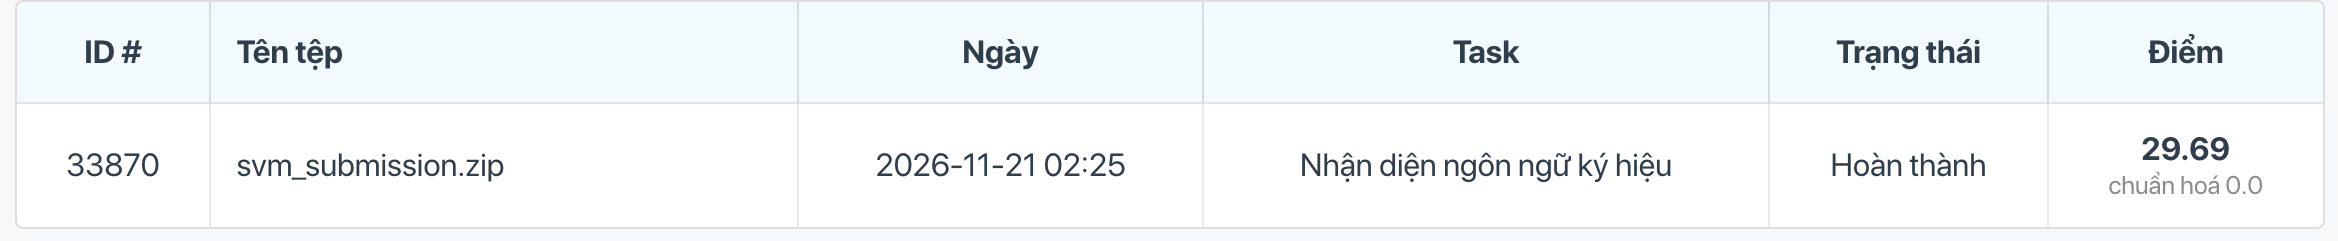
\includegraphics[width=\textwidth]{image/aichallenge/submissions_svm.png}
  \caption{Bài nộp của mô hình SVM ban đầu trên AIChallenge.}
  \label{fig:sub_svm}
\end{figure}

\begin{figure}[H]
  \centering
  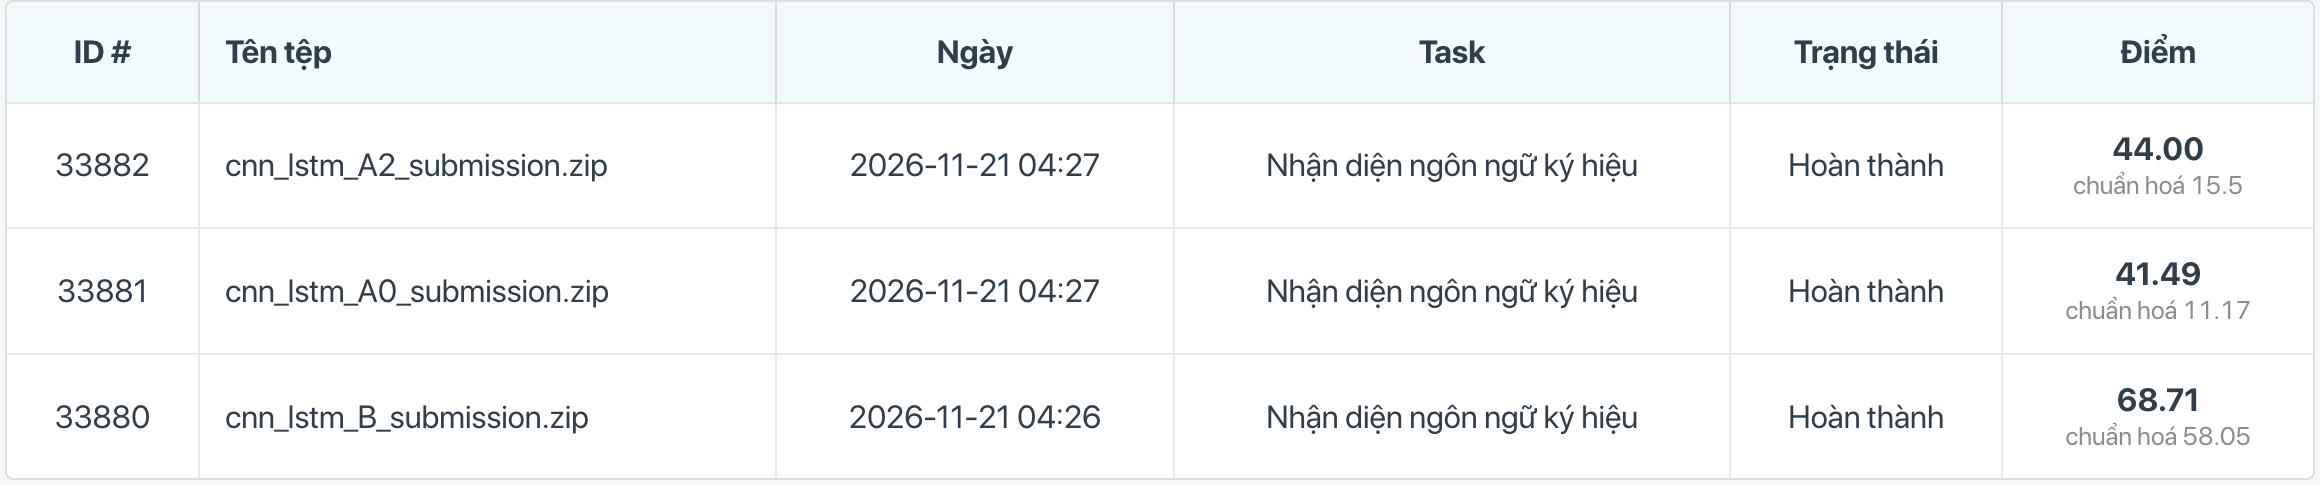
\includegraphics[width=\textwidth]{image/aichallenge/submissions_cnn_lstm.png}
  \caption{Các bài nộp của CNN-LSTM (A0, A2, B) trên AIChallenge.}
  \label{fig:sub_cnn_lstm}
\end{figure}

\begin{figure}[H]
  \centering
  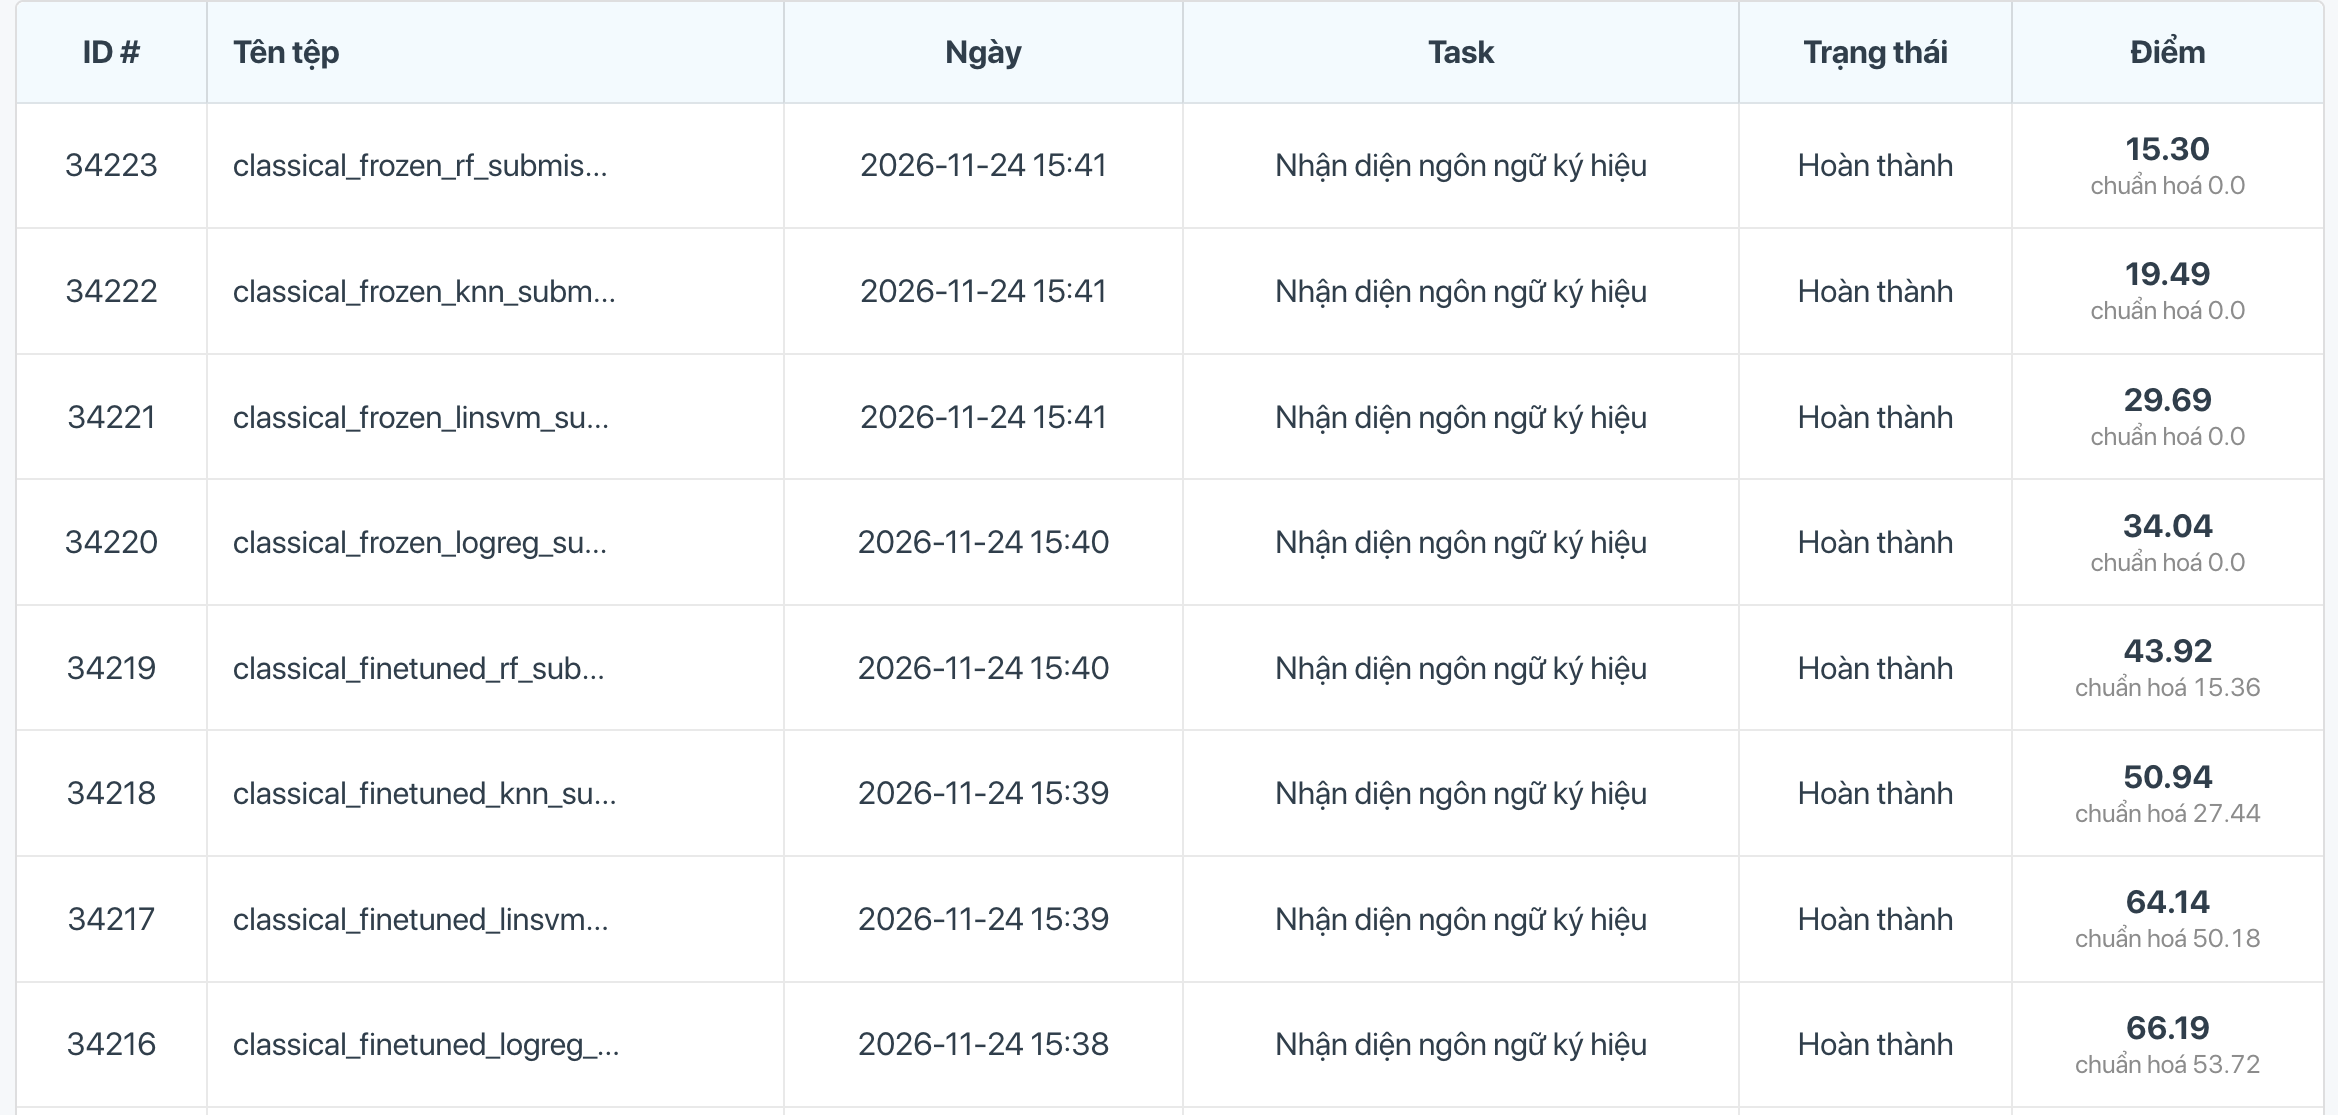
\includegraphics[width=\textwidth]{image/aichallenge/submissions_classical.png}
  \caption{Các bài nộp của bốn thuật toán cổ điển trên hai bộ đặc trưng trên AIChallenge.}
  \label{fig:sub_classical}
\end{figure}
